% ===========================================================================
%  TikuOS — TikuKits DS: State Machine for Embedded Systems
%  Beamer Presentation
% ===========================================================================
\documentclass[aspectratio=169, 10pt]{beamer}

% ---- Theme ----------------------------------------------------------------
\usetheme{Madrid}
\usecolortheme{whale}
\setbeamertemplate{navigation symbols}{}
\setbeamertemplate{footline}{%
  \leavevmode\hbox{%
    \begin{beamercolorbox}[wd=.33\paperwidth,ht=2.5ex,dp=1ex,center]{author in head/foot}%
      \usebeamerfont{author in head/foot}\insertshortauthor
    \end{beamercolorbox}%
    \begin{beamercolorbox}[wd=.34\paperwidth,ht=2.5ex,dp=1ex,center]{title in head/foot}%
      \usebeamerfont{title in head/foot}\insertshorttitle
    \end{beamercolorbox}%
    \begin{beamercolorbox}[wd=.33\paperwidth,ht=2.5ex,dp=1ex,right]{date in head/foot}%
      \usebeamerfont{date in head/foot}\insertshortdate{}\hspace*{2em}%
      \insertframenumber{}/\inserttotalframenumber\hspace*{2ex}
    \end{beamercolorbox}}%
  \vskip0pt%
}

% ---- Packages -------------------------------------------------------------
\usepackage{listings}
\usepackage{graphicx}
\usepackage{hyperref}
\usepackage{booktabs}
\usepackage{multirow}
\usepackage{tikz}
\usetikzlibrary{arrows.meta, positioning, shapes.geometric, calc,
                decorations.pathreplacing, fit}
\usepackage{amsmath}

% ---- Code listing style ---------------------------------------------------
\lstset{
  basicstyle=\ttfamily\scriptsize,
  keywordstyle=\color{blue}\bfseries,
  commentstyle=\color{gray},
  stringstyle=\color{red!70!black},
  showstringspaces=false,
  breaklines=true,
  frame=single,
  rulecolor=\color{black!30},
  backgroundcolor=\color{blue!3},
  tabsize=4,
}
\lstdefinestyle{cstyle}{
  language=C,
  morekeywords={uint8_t,uint16_t,uint32_t,int32_t,int16_t,bool,
                tiku_kits_ds_sm_t,tiku_kits_ds_sm_action_t,
                tiku_kits_ds_sm_transition_t,
                tiku_kits_ds_elem_t,
                TIKU_KITS_DS_OK,TIKU_KITS_DS_ERR_NULL,
                TIKU_KITS_DS_ERR_SIZE,TIKU_KITS_DS_ERR_PARAM,
                TIKU_KITS_DS_ERR_NOT_FOUND,
                TIKU_KITS_DS_SM_MAX_STATES,
                TIKU_KITS_DS_SM_MAX_EVENTS,
                TIKU_KITS_DS_SM_NO_TRANSITION,
                NULL},
}

% ---- Metadata -------------------------------------------------------------
\title[TikuKits DS]{TikuKits DS: State Machine for Embedded Systems}
\subtitle{Simple. Ubiquitous. Intelligence, Everywhere.}
\author[Ambuj Varshney]{Ambuj Varshney \\ \texttt{ambuj@tiku-os.org}}
\date{\today}

% ===========================================================================
\begin{document}

% ---------------------------------------------------------------------------
\begin{frame}
\titlepage
\end{frame}

% ---------------------------------------------------------------------------
\begin{frame}{Outline}
\tableofcontents
\end{frame}

% ===========================================================================
\section{Motivation}
% ===========================================================================

\begin{frame}{Why State Machines on MCUs?}
\begin{columns}[T]
\begin{column}{0.48\textwidth}
\begin{block}{The Problem}
\begin{itemize}
  \item Embedded systems have \textbf{modes}: idle, active, sleep, error
  \item Events trigger \textbf{transitions}: button press, timeout, fault
  \item Na\"{\i}ve approach: nested \texttt{if-else} / \texttt{switch}
  \item Grows into \textbf{unmaintainable spaghetti code}
\end{itemize}
\end{block}

\begin{block}{Embedded Use Cases}
\begin{itemize}
  \item \textbf{LED blink patterns} --- on/off/fade FSM
  \item \textbf{Communication protocols} --- UART/SPI handshake
  \item \textbf{Power management} --- active/LPM0/LPM3/LPM4
  \item \textbf{Sensor pipelines} --- init/sample/process/transmit
\end{itemize}
\end{block}
\end{column}

\begin{column}{0.48\textwidth}
\begin{center}
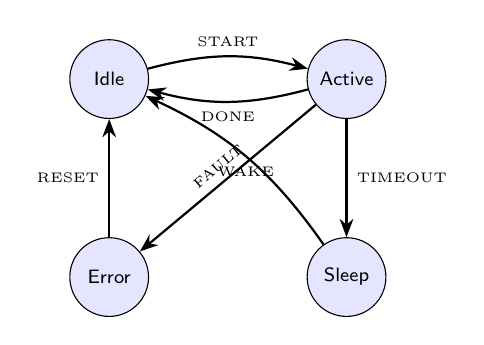
\begin{tikzpicture}[
    >=Stealth,
    state/.style={draw, circle, minimum size=1cm,
                  font=\scriptsize\sffamily, fill=blue!10},
    every edge/.style={draw, ->, thick},
    node distance=2cm
  ]
  \node[state] (idle) {Idle};
  \node[state, right=of idle] (active) {Active};
  \node[state, below=1.5cm of active] (sleep) {Sleep};
  \node[state, below=1.5cm of idle] (error) {Error};

  \draw[->] (idle) edge[bend left=15] node[above, font=\tiny] {START} (active);
  \draw[->] (active) edge[bend left=15] node[below, font=\tiny] {DONE} (idle);
  \draw[->] (active) edge node[right, font=\tiny] {TIMEOUT} (sleep);
  \draw[->] (sleep) edge[bend right=15] node[below, font=\tiny] {WAKE} (idle);
  \draw[->] (active) edge node[above, font=\tiny, sloped] {FAULT} (error);
  \draw[->] (error) edge node[left, font=\tiny] {RESET} (idle);
\end{tikzpicture}
\end{center}

\vspace{0.3em}
\begin{alertblock}{Design Goal}
A \textbf{table-driven} finite state machine: 2D array lookup
\texttt{table[state][event]} returns the next state and an
action callback. O(1) transitions, zero branching logic.
\end{alertblock}
\end{column}
\end{columns}
\end{frame}

% ===========================================================================
\section{Table-Driven FSM Theory}
% ===========================================================================

\begin{frame}[fragile]{Table-Driven vs.\ Switch-Case FSM}
\begin{columns}[T]
\begin{column}{0.48\textwidth}
\textbf{Switch-case approach (spaghetti):}
\begin{lstlisting}[style=cstyle, basicstyle=\ttfamily\tiny,
  title={The problem: nested switch-case}]
switch (state) {
  case IDLE:
    switch (event) {
      case START:
        start_motor();
        state = ACTIVE;
        break;
      case FAULT:
        log_error();
        state = ERROR;
        break;
      /* ... more cases ... */
    }
    break;
  case ACTIVE:
    switch (event) {
      /* ... even more cases ... */
    }
    break;
  /* ... grows unboundedly ... */
}
\end{lstlisting}

Every new state or event adds another branch.
Testing requires tracing every path.
\end{column}

\begin{column}{0.48\textwidth}
\textbf{Table-driven approach (clean):}
\begin{lstlisting}[style=cstyle, basicstyle=\ttfamily\tiny,
  title={The solution: 2D table lookup}]
/* Entire FSM logic in one line: */
transition = table[current_state][event];

if (transition.action != NULL)
    transition.action();

current_state = transition.next_state;
\end{lstlisting}

\vspace{0.5em}
\textbf{Advantages:}
\begin{itemize}
  \item All transitions visible in one table
  \item Adding states/events: just add rows/columns
  \item \textbf{Debuggable}: print \texttt{table[s][e]} to see any transition
  \item \textbf{Testable}: iterate all table entries
  \item \textbf{O(1)}: constant-time array indexing
  \item \textbf{No branching}: ideal for pipelined CPUs
\end{itemize}

\vspace{0.3em}
\begin{block}{Trade-Off}
Uses more memory (8$\times$8 table) but eliminates
all conditional logic. On MCUs, this is almost always
the right trade-off.
\end{block}
\end{column}
\end{columns}
\end{frame}

% ---------------------------------------------------------------------------
\begin{frame}{The Transition Table}
\begin{center}
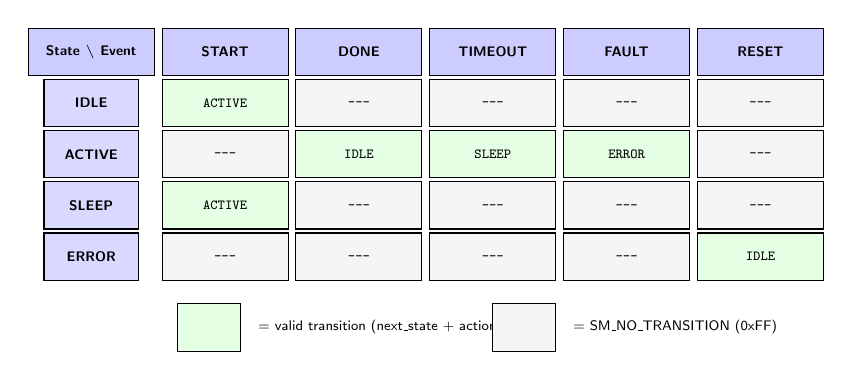
\begin{tikzpicture}[
    cell/.style={draw, minimum width=1.6cm, minimum height=0.6cm,
                 font=\tiny\ttfamily, text centered},
    hdr/.style={cell, fill=blue!20, font=\tiny\sffamily\bfseries},
    rhdr/.style={cell, fill=blue!15, font=\tiny\sffamily\bfseries,
                 minimum width=1.2cm},
    empty/.style={cell, fill=gray!8},
    valid/.style={cell, fill=green!10},
    >=Stealth
  ]
  % Column headers
  \node[hdr] at (0, 0) {State $\backslash$ Event};
  \node[hdr] at (1.7, 0) {START};
  \node[hdr] at (3.4, 0) {DONE};
  \node[hdr] at (5.1, 0) {TIMEOUT};
  \node[hdr] at (6.8, 0) {FAULT};
  \node[hdr] at (8.5, 0) {RESET};

  % Row 0: IDLE
  \node[rhdr] at (0, -0.65) {IDLE};
  \node[valid] at (1.7, -0.65) {ACTIVE};
  \node[empty] at (3.4, -0.65) {---};
  \node[empty] at (5.1, -0.65) {---};
  \node[empty] at (6.8, -0.65) {---};
  \node[empty] at (8.5, -0.65) {---};

  % Row 1: ACTIVE
  \node[rhdr] at (0, -1.3) {ACTIVE};
  \node[empty] at (1.7, -1.3) {---};
  \node[valid] at (3.4, -1.3) {IDLE};
  \node[valid] at (5.1, -1.3) {SLEEP};
  \node[valid] at (6.8, -1.3) {ERROR};
  \node[empty] at (8.5, -1.3) {---};

  % Row 2: SLEEP
  \node[rhdr] at (0, -1.95) {SLEEP};
  \node[valid] at (1.7, -1.95) {ACTIVE};
  \node[empty] at (3.4, -1.95) {---};
  \node[empty] at (5.1, -1.95) {---};
  \node[empty] at (6.8, -1.95) {---};
  \node[empty] at (8.5, -1.95) {---};

  % Row 3: ERROR
  \node[rhdr] at (0, -2.6) {ERROR};
  \node[empty] at (1.7, -2.6) {---};
  \node[empty] at (3.4, -2.6) {---};
  \node[empty] at (5.1, -2.6) {---};
  \node[empty] at (6.8, -2.6) {---};
  \node[valid] at (8.5, -2.6) {IDLE};

  % Legend
  \node[valid, minimum width=0.8cm] at (1.5, -3.5) {};
  \node[font=\tiny\sffamily, anchor=west] at (2.0, -3.5) {= valid transition (next\_state + action)};
  \node[empty, minimum width=0.8cm] at (5.5, -3.5) {};
  \node[font=\tiny\sffamily, anchor=west] at (6.0, -3.5) {= SM\_NO\_TRANSITION (0xFF)};
\end{tikzpicture}
\end{center}

\vspace{0.3em}
\begin{columns}[T]
\begin{column}{0.48\textwidth}
\begin{block}{Undefined Transitions}
\texttt{SM\_NO\_TRANSITION = 0xFF} means ``this event
is invalid in this state.'' The FSM stays in the
current state and takes no action.
\end{block}
\end{column}
\begin{column}{0.48\textwidth}
\begin{block}{Action Callbacks}
Each valid transition can optionally call an action function.
If \texttt{action == NULL}, no function is called but the
state change still occurs.
\end{block}
\end{column}
\end{columns}
\end{frame}

% ===========================================================================
\section{Data Structure}
% ===========================================================================

\begin{frame}[fragile]{The \texttt{tiku\_kits\_ds\_sm} Structure}
\begin{columns}[T]
\begin{column}{0.48\textwidth}
\begin{lstlisting}[style=cstyle,
  title={State machine structures}]
/* Action callback type */
typedef void (*tiku_kits_ds_sm_action_t)(void);

/* Single transition entry */
struct tiku_kits_ds_sm_transition {
    uint8_t next_state;
    tiku_kits_ds_sm_action_t action;
};

/* Full state machine */
struct tiku_kits_ds_sm {
    struct tiku_kits_ds_sm_transition
        table[TIKU_KITS_DS_SM_MAX_STATES]
             [TIKU_KITS_DS_SM_MAX_EVENTS];
    uint8_t current_state;
    uint8_t n_states;
    uint8_t n_events;
};
\end{lstlisting}
\end{column}

\begin{column}{0.48\textwidth}
\begin{lstlisting}[style=cstyle,
  title={Configuration macros}]
/* Maximum states and events */
#ifndef TIKU_KITS_DS_SM_MAX_STATES
#define TIKU_KITS_DS_SM_MAX_STATES  8
#endif

#ifndef TIKU_KITS_DS_SM_MAX_EVENTS
#define TIKU_KITS_DS_SM_MAX_EVENTS  8
#endif

/* Sentinel: undefined transition */
#define TIKU_KITS_DS_SM_NO_TRANSITION  0xFF
\end{lstlisting}

\vspace{0.3em}
\textbf{Memory footprint:}\\
Each transition: $1 + 2 = 3$ bytes (MSP430, 16-bit pointers).\\
Table: $8 \times 8 \times 3 = 192$ bytes.\\
Total: $192 + 3 = 195$ bytes.

\vspace{0.3em}
\begin{block}{Compact Design}
On 16-bit MSP430, function pointers are only 2 bytes.
The entire FSM fits in under 200 bytes of RAM.
\end{block}
\end{column}
\end{columns}
\end{frame}

% ===========================================================================
\section{API Reference}
% ===========================================================================

\begin{frame}[fragile]{Complete API}
\begin{table}
\centering
\small
\begin{tabular}{@{}lp{8cm}@{}}
\toprule
\textbf{Function} & \textbf{Description} \\
\midrule
\texttt{tiku\_kits\_ds\_sm\_init(sm, ns, ne)}
  & Initialize with \texttt{ns} states and \texttt{ne} events; all transitions set to \texttt{NO\_TRANSITION} \\
\texttt{tiku\_kits\_ds\_sm\_set\_transition(sm, s, e, ns, act)}
  & Define transition: in state \texttt{s} on event \texttt{e}, go to state \texttt{ns} and call \texttt{act} \\
\midrule
\texttt{tiku\_kits\_ds\_sm\_process(sm, event)}
  & Process event: lookup \texttt{table[current][event]}, call action, update state \\
\texttt{tiku\_kits\_ds\_sm\_get\_state(sm)}
  & Return current state index \\
\texttt{tiku\_kits\_ds\_sm\_set\_state(sm, s)}
  & Force state to \texttt{s} (no action called) \\
\midrule
\texttt{tiku\_kits\_ds\_sm\_reset(sm)}
  & Reset to state 0 (no action called) \\
\texttt{tiku\_kits\_ds\_sm\_clear(sm)}
  & Clear all transitions and reset state \\
\bottomrule
\end{tabular}
\end{table}

\vspace{0.3em}
\begin{alertblock}{The Core: process()}
\texttt{process()} is where all the magic happens. It performs a single
\texttt{table[current\_state][event]} lookup, calls the action callback
(if non-NULL), and updates the current state. Entire FSM logic
in \textbf{three lines of code}.
\end{alertblock}
\end{frame}

% ===========================================================================
\section{Internal Algorithm}
% ===========================================================================

\begin{frame}[fragile]{How process() Works}
\begin{columns}[T]
\begin{column}{0.52\textwidth}
\begin{lstlisting}[style=cstyle,
  title={The process function internals}]
int tiku_kits_ds_sm_process(
    struct tiku_kits_ds_sm *sm,
    uint8_t event)
{
    if (!sm)
        return TIKU_KITS_DS_ERR_NULL;
    if (event >= sm->n_events)
        return TIKU_KITS_DS_ERR_PARAM;

    /* Lookup transition */
    struct tiku_kits_ds_sm_transition *t =
        &sm->table[sm->current_state][event];

    /* Undefined transition? Stay put. */
    if (t->next_state ==
            TIKU_KITS_DS_SM_NO_TRANSITION)
        return TIKU_KITS_DS_ERR_NOT_FOUND;

    /* Call action callback (if any) */
    if (t->action != NULL)
        t->action();

    /* Update state */
    sm->current_state = t->next_state;

    return TIKU_KITS_DS_OK;
}
\end{lstlisting}
\end{column}

\begin{column}{0.44\textwidth}
\begin{center}
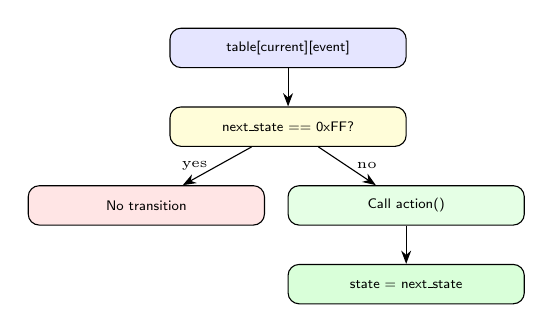
\begin{tikzpicture}[
    box/.style={draw, rounded corners, minimum width=3cm,
                minimum height=0.5cm, font=\tiny\sffamily,
                text centered},
    >=Stealth
  ]
  \node[box, fill=blue!10] (lookup) at (0, 3.5) {table[current][event]};
  \node[box, fill=yellow!15] (check) at (0, 2.5) {next\_state == 0xFF?};
  \node[box, fill=red!10] (noop) at (-1.8, 1.5) {No transition};
  \node[box, fill=green!10] (action) at (1.5, 1.5) {Call action()};
  \node[box, fill=green!15] (update) at (1.5, 0.5) {state = next\_state};

  \draw[->] (lookup) -- (check);
  \draw[->] (check) -- node[left, font=\tiny] {yes} (noop);
  \draw[->] (check) -- node[right, font=\tiny] {no} (action);
  \draw[->] (action) -- (update);
\end{tikzpicture}
\end{center}

\vspace{0.3em}
\begin{block}{O(1) Guaranteed}
No loops, no comparisons against state lists.
Just one array index operation plus a function
pointer call. Constant time regardless of how
many states or events exist.
\end{block}
\end{column}
\end{columns}
\end{frame}

% ---------------------------------------------------------------------------
\begin{frame}[fragile]{Setting Up Transitions}
\begin{columns}[T]
\begin{column}{0.52\textwidth}
\begin{lstlisting}[style=cstyle,
  title={Building the transition table}]
int tiku_kits_ds_sm_set_transition(
    struct tiku_kits_ds_sm *sm,
    uint8_t state,
    uint8_t event,
    uint8_t next_state,
    tiku_kits_ds_sm_action_t action)
{
    if (!sm)
        return TIKU_KITS_DS_ERR_NULL;
    if (state >= sm->n_states ||
        event >= sm->n_events ||
        next_state >= sm->n_states)
        return TIKU_KITS_DS_ERR_PARAM;

    sm->table[state][event].next_state =
        next_state;
    sm->table[state][event].action =
        action;

    return TIKU_KITS_DS_OK;
}
\end{lstlisting}
\end{column}

\begin{column}{0.44\textwidth}
\textbf{Validation:}
\begin{itemize}
  \item State index must be $< n\_states$
  \item Event index must be $< n\_events$
  \item Next state must be $< n\_states$
  \item Action can be \texttt{NULL} (no-op transition)
\end{itemize}

\vspace{0.5em}
\begin{block}{Init Fills NO\_TRANSITION}
\texttt{init()} sets every \texttt{next\_state} to
\texttt{0xFF} and every \texttt{action} to \texttt{NULL}.
Only explicitly defined transitions are valid.
This is a fail-safe default: unknown events are
silently ignored.
\end{block}

\vspace{0.3em}
\begin{alertblock}{Build Then Run}
Define all transitions with \texttt{set\_transition()}
\textbf{before} calling \texttt{process()}. The table
is not locked --- transitions can be changed at runtime
for adaptive behavior.
\end{alertblock}
\end{column}
\end{columns}
\end{frame}

% ===========================================================================
\section{Examples}
% ===========================================================================

\begin{frame}[fragile]{Example 1: LED Blink Pattern FSM}
\begin{lstlisting}[style=cstyle,
  title={examples/example\_ds\_sm.c --- LED blink controller}]
/* States */
enum { LED_OFF = 0, LED_ON = 1, LED_BLINK = 2, N_STATES = 3 };
/* Events */
enum { EVT_PRESS = 0, EVT_TIMER = 1, EVT_LONG_PRESS = 2, N_EVENTS = 3 };

/* Action callbacks */
void action_led_on(void)  { P1OUT |= BIT0; }
void action_led_off(void) { P1OUT &= ~BIT0; }
void action_toggle(void)  { P1OUT ^= BIT0; }

struct tiku_kits_ds_sm led_sm;

void setup_led_fsm(void) {
    tiku_kits_ds_sm_init(&led_sm, N_STATES, N_EVENTS);

    /* OFF + PRESS -> ON (turn LED on) */
    tiku_kits_ds_sm_set_transition(&led_sm, LED_OFF, EVT_PRESS, LED_ON, action_led_on);
    /* ON + PRESS -> OFF (turn LED off) */
    tiku_kits_ds_sm_set_transition(&led_sm, LED_ON, EVT_PRESS, LED_OFF, action_led_off);
    /* ON + LONG_PRESS -> BLINK (start blinking) */
    tiku_kits_ds_sm_set_transition(&led_sm, LED_ON, EVT_LONG_PRESS, LED_BLINK, action_toggle);
    /* BLINK + TIMER -> BLINK (toggle on each tick) */
    tiku_kits_ds_sm_set_transition(&led_sm, LED_BLINK, EVT_TIMER, LED_BLINK, action_toggle);
    /* BLINK + PRESS -> OFF (stop blinking) */
    tiku_kits_ds_sm_set_transition(&led_sm, LED_BLINK, EVT_PRESS, LED_OFF, action_led_off);
}
\end{lstlisting}
\end{frame}

% ---------------------------------------------------------------------------
\begin{frame}[fragile]{Example 1 (cont.): Running the LED FSM}
\begin{columns}[T]
\begin{column}{0.52\textwidth}
\begin{lstlisting}[style=cstyle,
  title={Processing events in the main loop}]
void main(void) {
    setup_led_fsm();

    while (1) {
        uint8_t event = get_event();

        tiku_kits_ds_sm_process(
            &led_sm, event);

        /* Check current state */
        uint8_t s =
            tiku_kits_ds_sm_get_state(
                &led_sm);

        if (s == LED_BLINK) {
            /* Arm timer for next toggle */
            start_blink_timer();
        }

        /* Enter LPM until next event */
        __bis_SR_register(LPM3_bits);
    }
}
\end{lstlisting}
\end{column}

\begin{column}{0.44\textwidth}
\begin{center}
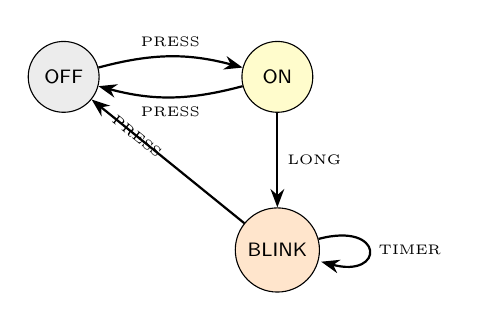
\begin{tikzpicture}[
    >=Stealth,
    state/.style={draw, circle, minimum size=0.9cm,
                  font=\scriptsize\sffamily, fill=blue!10},
    every edge/.style={draw, ->, thick},
    node distance=1.8cm
  ]
  \node[state, fill=gray!15] (off) {OFF};
  \node[state, fill=yellow!20, right=of off] (on) {ON};
  \node[state, fill=orange!20, below=1.2cm of on] (blink) {BLINK};

  \draw[->] (off) edge[bend left=15]
    node[above, font=\tiny] {PRESS} (on);
  \draw[->] (on) edge[bend left=15]
    node[below, font=\tiny] {PRESS} (off);
  \draw[->] (on) edge
    node[right, font=\tiny] {LONG} (blink);
  \draw[->] (blink) edge[loop right]
    node[right, font=\tiny] {TIMER} (blink);
  \draw[->] (blink) edge
    node[left, font=\tiny, sloped] {PRESS} (off);
\end{tikzpicture}
\end{center}

\vspace{0.5em}
\begin{block}{Self-Transitions}
\texttt{BLINK + TIMER $\rightarrow$ BLINK} is a self-transition.
The action (\texttt{toggle}) executes, but the state stays
the same. This is how periodic behaviors work.
\end{block}
\end{column}
\end{columns}
\end{frame}

% ---------------------------------------------------------------------------
\begin{frame}[fragile]{Example 2: Communication Protocol Handler}
\begin{columns}[T]
\begin{column}{0.52\textwidth}
\begin{lstlisting}[style=cstyle,
  title={UART protocol state machine}]
/* States */
enum { ST_IDLE, ST_HEADER, ST_PAYLOAD,
       ST_CHECKSUM, N_PROTO_STATES };
/* Events */
enum { EVT_BYTE_RX, EVT_VALID, EVT_INVALID,
       EVT_COMPLETE, N_PROTO_EVENTS };

void action_store_header(void) {
    proto_buf.header = uart_rx_byte;
    proto_buf.idx = 0;
}
void action_store_byte(void) {
    proto_buf.data[proto_buf.idx++] =
        uart_rx_byte;
}
void action_verify(void) {
    compute_checksum(&proto_buf);
}
void action_dispatch(void) {
    process_packet(&proto_buf);
}

/* Setup transitions */
set_transition(&proto_sm, ST_IDLE,
    EVT_BYTE_RX, ST_HEADER,
    action_store_header);
set_transition(&proto_sm, ST_HEADER,
    EVT_BYTE_RX, ST_PAYLOAD,
    action_store_byte);
/* ... */
\end{lstlisting}
\end{column}

\begin{column}{0.44\textwidth}
\begin{center}
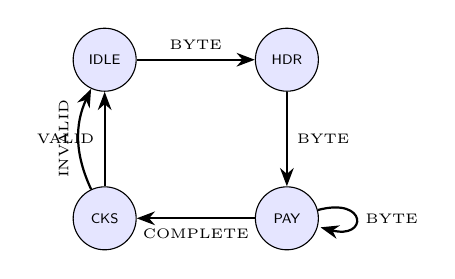
\begin{tikzpicture}[
    >=Stealth,
    state/.style={draw, circle, minimum size=0.8cm,
                  font=\tiny\sffamily, fill=blue!10},
    every edge/.style={draw, ->, thick},
    node distance=1.5cm
  ]
  \node[state] (idle) {IDLE};
  \node[state, right=of idle] (hdr) {HDR};
  \node[state, below=1.2cm of hdr] (pay) {PAY};
  \node[state, below=1.2cm of idle] (chk) {CKS};

  \draw[->] (idle) edge node[above, font=\tiny] {BYTE} (hdr);
  \draw[->] (hdr) edge node[right, font=\tiny] {BYTE} (pay);
  \draw[->] (pay) edge[loop right]
    node[right, font=\tiny] {BYTE} (pay);
  \draw[->] (pay) edge node[below, font=\tiny] {COMPLETE} (chk);
  \draw[->] (chk) edge node[left, font=\tiny] {VALID} (idle);
  \draw[->] (chk) edge[bend left=25] node[above, font=\tiny, sloped] {INVALID} (idle);
\end{tikzpicture}
\end{center}

\vspace{0.3em}
\begin{block}{Protocol Parsing}
Each received byte generates an event.
The FSM handles framing, payload accumulation,
and checksum verification --- all via table lookup.
No parsing logic in the ISR.
\end{block}

\vspace{0.3em}
\begin{alertblock}{ISR-Safe}
\texttt{process()} can be called directly from a
UART RX interrupt. The O(1) execution time is
bounded and deterministic.
\end{alertblock}
\end{column}
\end{columns}
\end{frame}

% ---------------------------------------------------------------------------
\begin{frame}[fragile]{Example 3: Power Management States}
\begin{columns}[T]
\begin{column}{0.52\textwidth}
\begin{lstlisting}[style=cstyle,
  title={MSP430 power state management}]
/* States */
enum { PWR_ACTIVE, PWR_LPM0, PWR_LPM3,
       PWR_LPM4, N_PWR_STATES };
/* Events */
enum { EVT_IDLE, EVT_DEEP_IDLE,
       EVT_SHUTDOWN, EVT_WAKEUP,
       N_PWR_EVENTS };

void enter_lpm0(void) {
    __bis_SR_register(LPM0_bits + GIE);
}
void enter_lpm3(void) {
    __bis_SR_register(LPM3_bits + GIE);
}
void enter_lpm4(void) {
    __bis_SR_register(LPM4_bits + GIE);
}
void exit_lpm(void) {
    __bic_SR_register_on_exit(
        LPM4_bits);
}

/* ACTIVE + IDLE -> LPM0 */
/* ACTIVE + DEEP_IDLE -> LPM3 */
/* LPM0 + DEEP_IDLE -> LPM3 */
/* LPMx + WAKEUP -> ACTIVE */
/* ACTIVE + SHUTDOWN -> LPM4 */
\end{lstlisting}
\end{column}

\begin{column}{0.44\textwidth}
\begin{center}
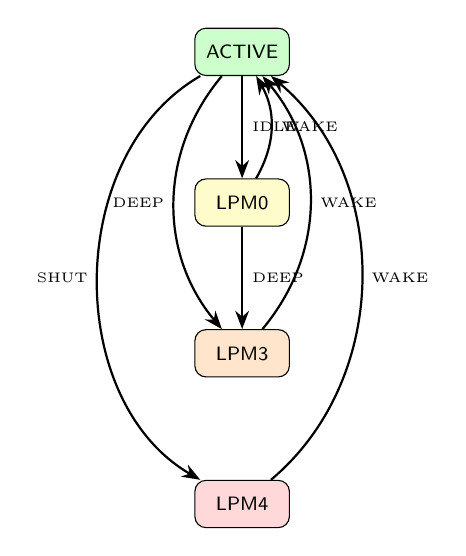
\begin{tikzpicture}[
    >=Stealth,
    state/.style={draw, rounded corners, minimum width=1.2cm,
                  minimum height=0.6cm, font=\scriptsize\sffamily,
                  text centered},
    every edge/.style={draw, ->, thick},
    node distance=1.3cm
  ]
  \node[state, fill=green!20] (active) {ACTIVE};
  \node[state, fill=yellow!20, below=of active] (lpm0) {LPM0};
  \node[state, fill=orange!20, below=of lpm0] (lpm3) {LPM3};
  \node[state, fill=red!15, below=of lpm3] (lpm4) {LPM4};

  \draw[->] (active) edge node[right, font=\tiny] {IDLE} (lpm0);
  \draw[->] (active) edge[bend right=40]
    node[left, font=\tiny] {DEEP} (lpm3);
  \draw[->] (lpm0) edge node[right, font=\tiny] {DEEP} (lpm3);
  \draw[->] (active) edge[bend right=60]
    node[left, font=\tiny] {SHUT} (lpm4);

  \draw[->] (lpm0) edge[bend right=30]
    node[right, font=\tiny] {WAKE} (active);
  \draw[->] (lpm3) edge[bend right=40]
    node[right, font=\tiny] {WAKE} (active);
  \draw[->] (lpm4) edge[bend right=50]
    node[right, font=\tiny] {WAKE} (active);
\end{tikzpicture}
\end{center}

\vspace{0.3em}
\begin{block}{Power Hierarchy}
The FSM enforces valid power transitions.
You cannot jump from LPM4 to LPM0 directly ---
you must wake to ACTIVE first. The table
simply has no transition defined for that case.
\end{block}
\end{column}
\end{columns}
\end{frame}

% ===========================================================================
\section{Comparison: FSM vs.\ If-Else}
% ===========================================================================

\begin{frame}{FSM vs.\ Switch-Case: Quantified}
\begin{table}
\centering
\small
\begin{tabular}{@{}lcc@{}}
\toprule
\textbf{Property} & \textbf{Table-Driven FSM} & \textbf{Switch-Case FSM} \\
\midrule
Transition time       & O(1) --- array lookup     & O($s \times e$) --- branch chain \\
Code size growth      & O(1) per transition        & O($s \times e$) branches \\
Adding a state        & One row in table           & Touch every switch block \\
Adding an event       & One column in table        & Touch every state handler \\
Debuggability         & Print table entry           & Step through branches \\
Testability           & Iterate all entries         & Cover all paths \\
Memory (4s, 4e)       & $4\times4\times3 = 48$\,B  & $\sim$100--200\,B code \\
ISR-safe              & Yes (deterministic time)    & Maybe (depends on branches) \\
\bottomrule
\end{tabular}
\end{table}

\vspace{0.5em}
\begin{columns}[T]
\begin{column}{0.48\textwidth}
\begin{block}{Not a Data Structure?}
Correct --- a state machine is not a classic data structure
like a stack or queue. But it is \textbf{fundamental to every
embedded system}. The table-driven implementation is essentially
a 2D array with structured lookup.
\end{block}
\end{column}

\begin{column}{0.48\textwidth}
\begin{block}{When Switch-Case Wins}
\begin{itemize}
  \item Only 2--3 states, 1--2 events
  \item Transitions need complex logic (not just callbacks)
  \item Memory is so tight even 48 bytes matters
\end{itemize}
\end{block}
\end{column}
\end{columns}
\end{frame}

% ===========================================================================
\section{Test Suite}
% ===========================================================================

\begin{frame}{Test Cases Overview}
\begin{table}
\centering
\small
\begin{tabular}{@{}clp{7cm}@{}}
\toprule
\textbf{\#} & \textbf{Test Function} & \textbf{What It Verifies} \\
\midrule
1 & \texttt{test\_kits\_ds\_sm\_init}
  & All transitions set to \texttt{NO\_TRANSITION}, state = 0 \\
2 & \texttt{test\_kits\_ds\_sm\_set\_transition}
  & Transition stored correctly in table \\
3 & \texttt{test\_kits\_ds\_sm\_process\_basic}
  & State changes correctly on valid event \\
4 & \texttt{test\_kits\_ds\_sm\_action\_called}
  & Action callback is invoked during transition \\
5 & \texttt{test\_kits\_ds\_sm\_no\_transition}
  & Undefined transitions return \texttt{ERR\_NOT\_FOUND}, state unchanged \\
6 & \texttt{test\_kits\_ds\_sm\_null\_action}
  & Transition with NULL action changes state without crash \\
7 & \texttt{test\_kits\_ds\_sm\_self\_transition}
  & Self-loop calls action, state stays same \\
8 & \texttt{test\_kits\_ds\_sm\_get\_set\_state}
  & \texttt{get\_state} and \texttt{set\_state} work correctly \\
9 & \texttt{test\_kits\_ds\_sm\_reset\_clear}
  & Reset returns to state 0; clear wipes all transitions \\
10 & \texttt{test\_kits\_ds\_sm\_null\_inputs}
  & All functions reject NULL with \texttt{ERR\_NULL} \\
\bottomrule
\end{tabular}
\end{table}
\end{frame}

% ===========================================================================
\section{Embedded Considerations}
% ===========================================================================

\begin{frame}{Embedded Design Patterns}
\begin{columns}[T]
\begin{column}{0.48\textwidth}
\begin{block}{Runtime Reconfiguration}
\begin{itemize}
  \item Transitions can be changed at runtime
  \item Swap action callbacks for different modes
  \item Add/remove transitions dynamically
  \item Useful for adaptive protocols
\end{itemize}
\end{block}

\begin{block}{Multiple FSMs}
\begin{itemize}
  \item Instantiate multiple \texttt{tiku\_kits\_ds\_sm} structs
  \item Each manages an independent concern
  \item LED FSM + Protocol FSM + Power FSM
  \item All share the same API
\end{itemize}
\end{block}
\end{column}

\begin{column}{0.48\textwidth}
\begin{block}{Integration with TikuOS}
\begin{itemize}
  \item Process events map to FSM events
  \item Timer callbacks trigger FSM transitions
  \item ISR posts event $\rightarrow$ process calls \texttt{process()}
  \item FSM actions post events to other processes
\end{itemize}
\end{block}

\begin{block}{Debugging}
\begin{lstlisting}[style=cstyle, basicstyle=\ttfamily\tiny]
/* Log every transition */
uint8_t old = tiku_kits_ds_sm_get_state(&sm);
tiku_kits_ds_sm_process(&sm, event);
uint8_t new_s = tiku_kits_ds_sm_get_state(&sm);
if (old != new_s) {
    uart_printf("FSM: %d -> %d (evt %d)",
                old, new_s, event);
}
\end{lstlisting}
\end{block}
\end{column}
\end{columns}
\end{frame}

% ===========================================================================
\section{Summary}
% ===========================================================================

\begin{frame}{Summary}
\begin{columns}[T]
\begin{column}{0.48\textwidth}
\begin{block}{What We Built}
\begin{itemize}
  \item Table-driven finite state machine
  \item 2D array: \texttt{table[state][event]}
  \item O(1) transitions via array indexing
  \item Action callbacks as function pointers
  \item 195 bytes state (8 states, 8 events)
  \item \texttt{NO\_TRANSITION} sentinel for safety
\end{itemize}
\end{block}

\begin{block}{Key Design Choices}
\begin{itemize}
  \item \texttt{0xFF} marks undefined transitions
  \item NULL action allowed (state-only transition)
  \item Self-transitions supported
  \item Validation on all inputs
\end{itemize}
\end{block}
\end{column}

\begin{column}{0.48\textwidth}
\begin{block}{Use Cases}
\begin{itemize}
  \item LED blink pattern controller
  \item Communication protocol handler
  \item Power management state machine
  \item Sensor pipeline orchestration
\end{itemize}
\end{block}

\begin{block}{Files}
\scriptsize
\begin{tabular}{@{}lp{4.5cm}@{}}
Header: & \texttt{ds/fsm/tiku\_kits\_ds\_sm.h} \\
Source: & \texttt{ds/fsm/tiku\_kits\_ds\_sm.c} \\
Tests: & \texttt{tests/ds/test\_kits\_ds\_sm.c} \\
Example: & \texttt{examples/example\_ds\_sm.c} \\
\end{tabular}
\end{block}
\end{column}
\end{columns}
\end{frame}

% ---------------------------------------------------------------------------
\begin{frame}{Thank You}
\begin{center}
\Large\textbf{TikuKits DS: State Machine}\\[0.5em]
\normalsize Table-Driven FSM for Resource-Constrained Endpoints\\[1.5em]

\begin{tabular}{rl}
  Repository: & \url{https://github.com/tikuos/tikuOS} \\
  License:    & Apache 2.0 \\
  Common:     & \texttt{tikukits/ds/tiku\_kits\_ds.h} \\
  Header:     & \texttt{tikukits/ds/fsm/tiku\_kits\_ds\_sm.h} \\
  Source:     & \texttt{tikukits/ds/fsm/tiku\_kits\_ds\_sm.c} \\
  Tests:      & \texttt{tikukits/tests/ds/test\_kits\_ds\_sm.c} \\
  Examples:   & \texttt{tikukits/examples/example\_ds\_sm.c} \\
\end{tabular}
\end{center}
\end{frame}

\end{document}
